\chapter{Arhitektura korisnog tereta FERSAT-a} \label{chapter:arhitektura}

Tipična arhitektura nanosatelita CubeSat sastoji se od dva dijela: platforme \engl{bus} i korisnog tereta \engl{payload}. Platformu čine svi oni sustavi koji su nužni za održavanje satelita u orbiti i njegov ispravan rad, primjerice sustav napajanja sa solarnim panelima, sustav za upravljanje položajem i orijentacijom satelita, komunikacijski sustav za slanje telemetrijskih podataka, i drugi. Većina CubeSat satelita koriste iste ili vrlo slične platforme, pa su gotova rješenja komercijalno dostupna. Korisni teret sadrži sustave koji služe za ispunjavanje primarne zadaće satelita. Budući da svaki satelit ima drugačiju zadaću, korisni teret mora biti razvijen posebno za određeni satelit.

Planirani korisni teret \engl{payload} FERSAT-a podijeljen je na tri podsustava:

\begin{itemize}
    \item kamera za snimanje površine Zemlje i zemaljskog horizonta,
    \item detektori svjetla u vidljivom i ultraljubičastom dijelu spektra za mjerenje svjetlosnog onečišćenja i debljine stupca ozona,
    \item komunikacijski sustav u radijskom X-pojasu (10.45 GHz) za prijenos podataka na Zemlju.
\end{itemize}

Radom korisnog tereta upravlja \textit{Payload Data Handler} (PDH) računalo. Zadaća je PDH računala prikupiti podatke iz senzorskog podsustava i kamere, pohraniti ih u trajnu memoriju \engl{non-volatile memory} te poslati prikupljene podatke na Zemlju korištenjem komunikacijskog podsustava. Kao PDH računalo odabran je mikrokontroler STM32L471VGT6 proizvođača ST Microelectronics.

Za rad ostalih podsustava satelita koji nisu direktno vezani uz koristan teret brine se \textit{Command and Data Handler} (CDH) računalo. CDH računalo također upravlja napajanjem korisnog tereta i šalje naredbe PDH računalu. Komunikacija CDH i PDH računala odvija se korištenjem sučelja CAN (\textit{Controller Area Network}). Konkretno CDH računalo u trenutku pisanja ovog teksta još nije odabrano. Slika \ref{fig:fersat_blok} prikazuje blok dijagram cijelog sustava.

\begin{figure}[htb]
    \centering
    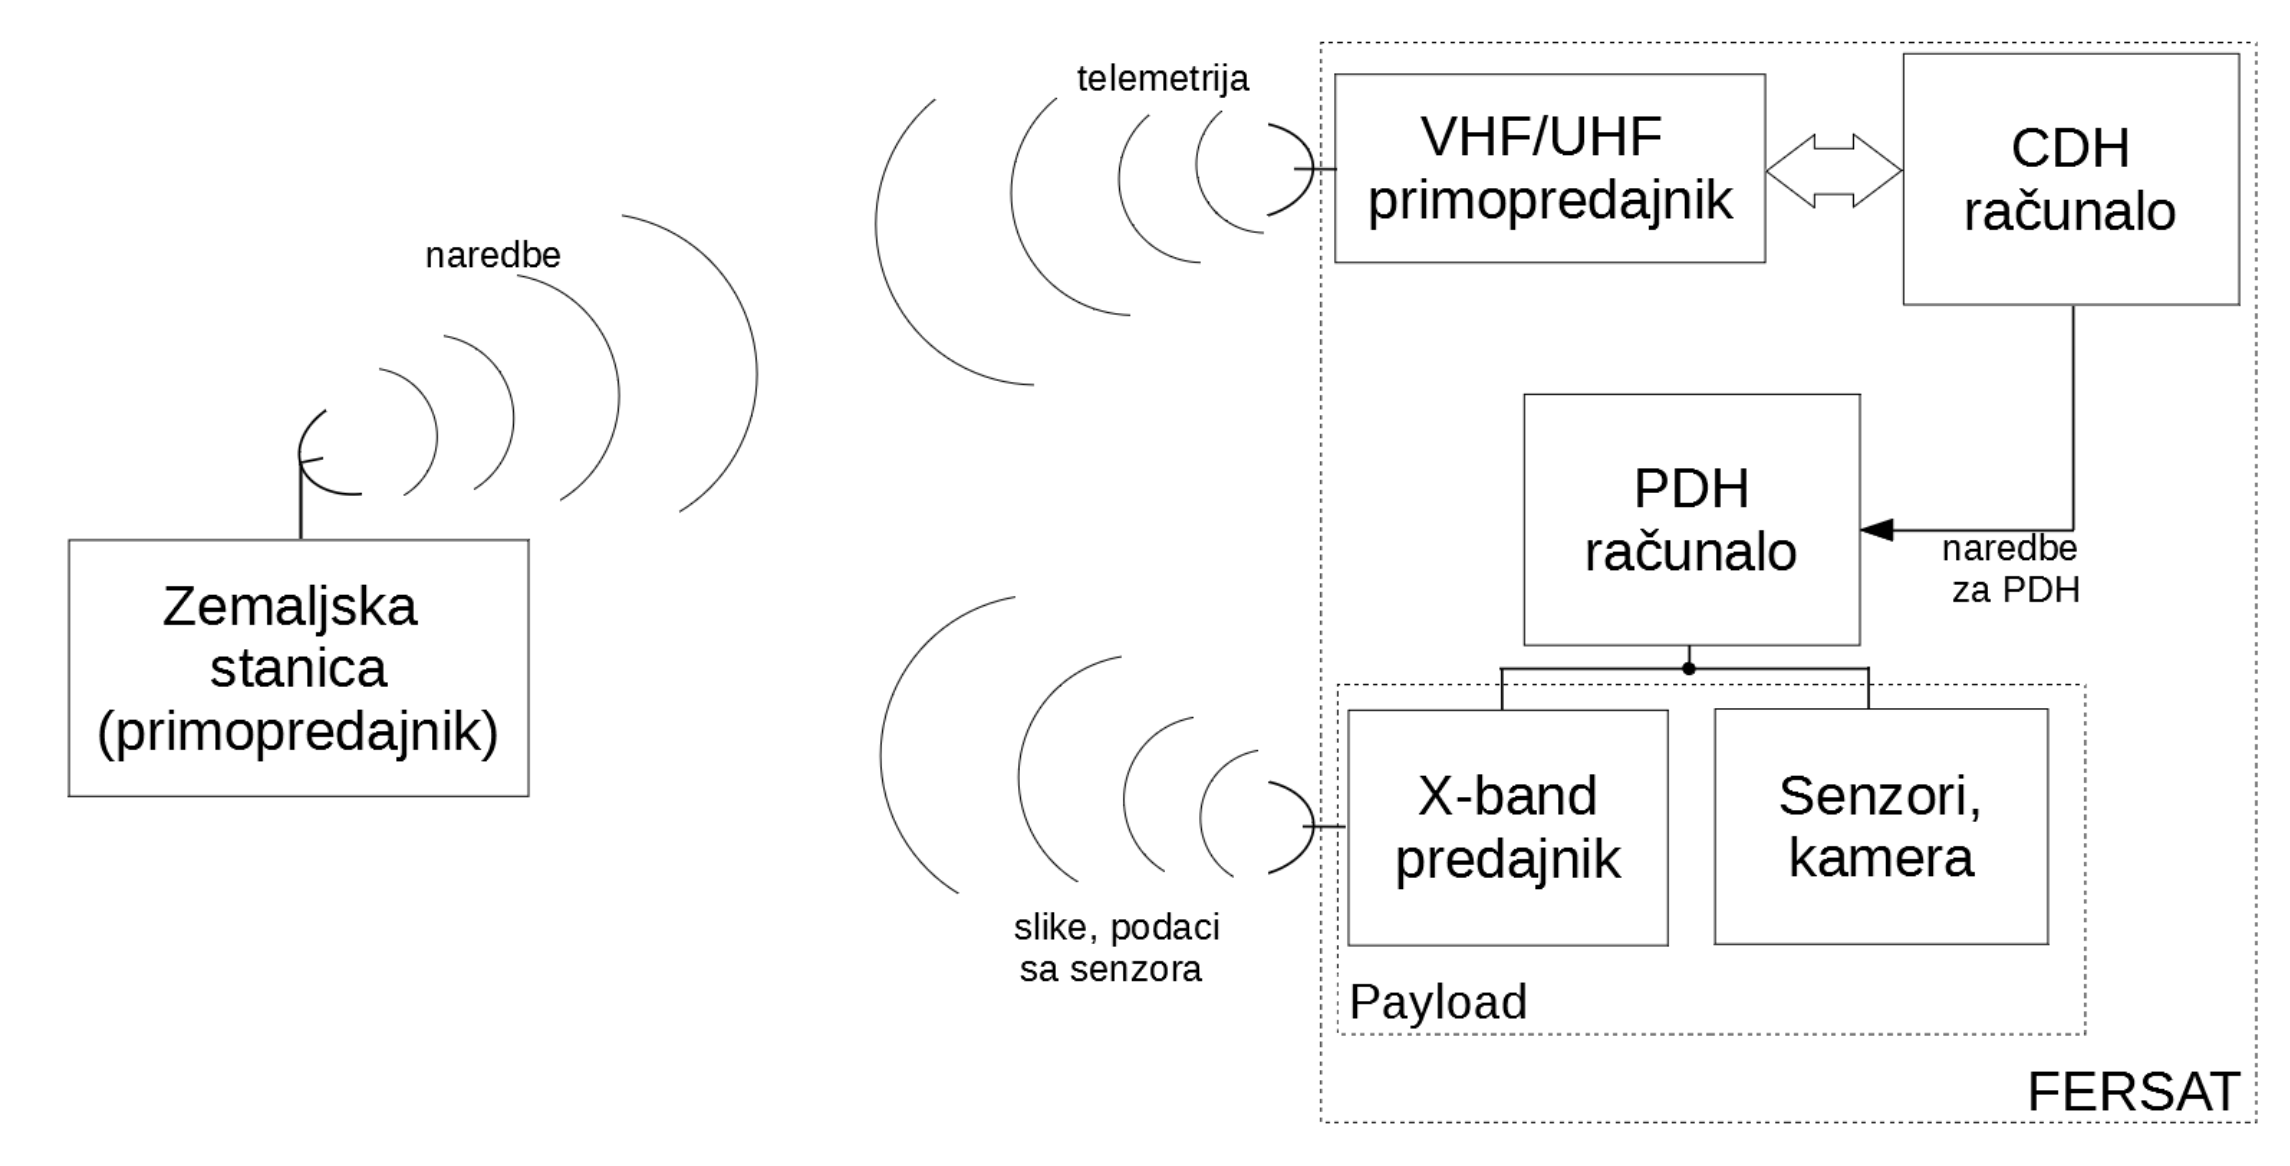
\includegraphics[width=\textwidth]{slike/fersat_blok_dijagram.png}
    \caption{Blok dijagram FERSAT-a i komunikacija sa zemaljskom postajom \cite{diplomski_goran_petrak}}
    \label{fig:fersat_blok}
\end{figure}

Senzorski podsustav ima dvije temeljne zadaće. Prva od njih je korištenjem fotosenzora koji rade u vidljivom dijelu elektromagnetskog spektra prikupiti podatke na temelju kojih će biti moguće odrediti udio LED rasvjete u naseljenim mjestima u odnosu na konvencionalnu natrijevu, metal-halidnu i fluorescentnu javnu rasvjetu. U sklopu projekta FERSAT već je razvijen algoritam koji na temelju obrade signala multispektralnog svjetla sa Zemlje može odrediti ovu informaciju \cite{diplomski_jakov_tutavac}. Mjerenje udjela LED rasvjete zanimljivo je zbog mogućih negativnih utjecaja plavog svjetla na ljudsko zdravlje, koje LED rasvjeta emitira u znatno većem intenzitetu nego konvencionalna \cite{falchi_light_pollution}.

Druga je zadaća senzorskog podsustava mjerenje propusnosti i refleksije atmosfere za ultraljubičasto svjetlo u svrhu određivanja debljine ozonskog omotača. Za mjerenje se koriste PureB detektori ultraljubičastog zračenja razvijeni na FER-u \cite{diplomski_filip_bogdanovic} i algoritmi razvijeni za tu namjenu \cite{zavrsni_kristian_stepancic}. Uspješna mjerenja po prvi put bi potvrdila mogućnost korištenja ove tehnologije u mjerenjima debljine ozonskog omotača iz svemira.

Upravljačko sklopovlje potrebno za rad PDH računala već je razvijeno \cite{zavrsni_filip_juric}. Tiskana pločica PDH računala, osim mikrokontrolera STM32L471VGT6, sadrži i vanjsku \textit{Flash} memoriju, sustav za napajanje, sklop za kontrolu izvođenja programa \engl{watchdog}, upravljački sklop za CAN komunikaciju i konektore za povezivanje s ostalim dijelovima sustava. PDH pločica bit će smještena ispod senzorske pločice, u takozvanoj \textit{stack-up} konfiguraciji (slika \ref{fig:fersat_3d}).

\begin{figure}[htb]
    \centering
    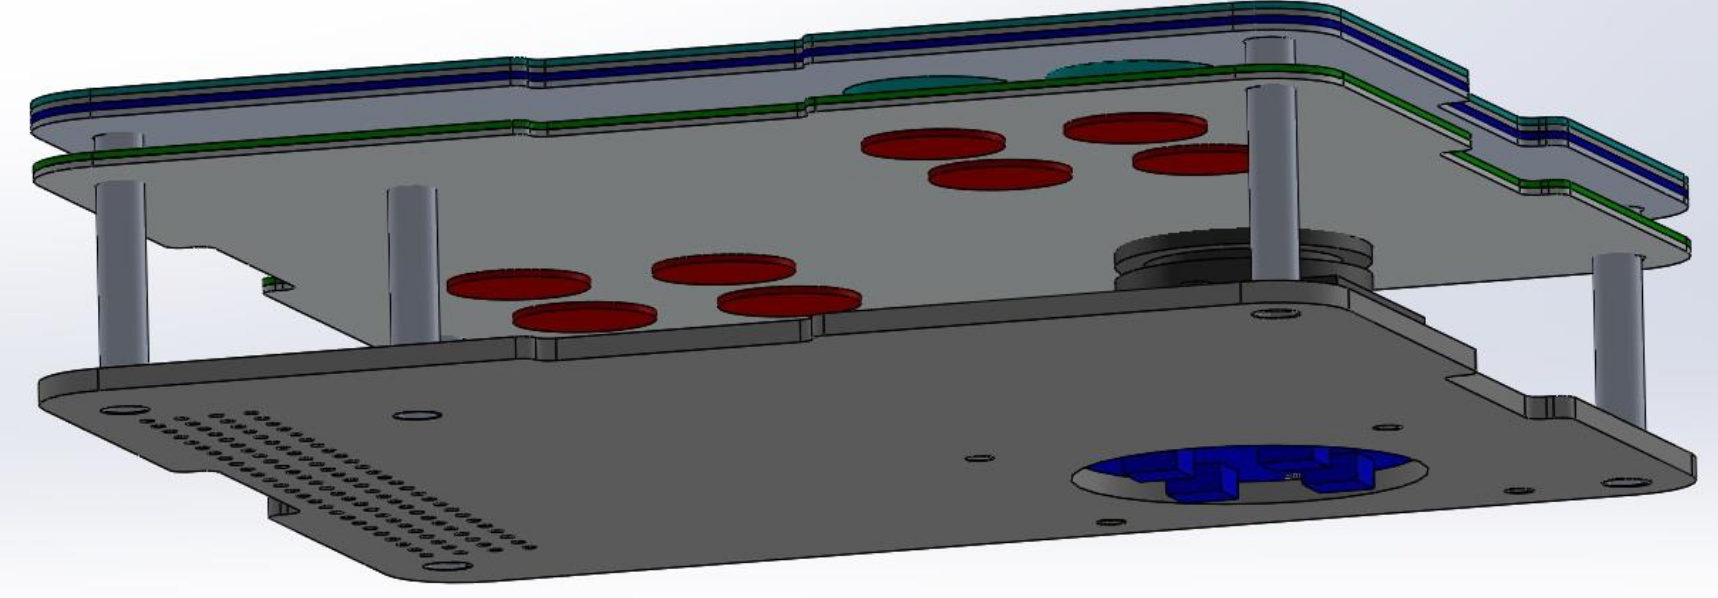
\includegraphics[width=\textwidth]{slike/fersat_3d.png}
    \caption{Trodimenzionalni model korisnog tereta FERSAT-a. PDH računalo smješteno je na donjoj pločici, a senzorski podsustav na srednjoj \cite{zavrsni_filip_juric}}
    \label{fig:fersat_3d}
\end{figure}

Također, u sklopu projekta FERSAT razvijen je i dio programske potpore PDH računala \cite{diplomski_goran_petrak}. No, kako je u međuvremenu došlo do promjene izbora mikrokontrolera PDH računala i promjene dijela sklopovlja senzorskog podsustava, dijelove te programske potpore bilo je potrebno prilagoditi ili ponovno razviti.

Prethodno razvijena programska potpora koristi operacijski sustav za rad u stvarnom vremenu FreeRTOS. Raspodjela poslova u FreeRTOS-u obavlja se korištenjem takozvanih zadataka \engl{tasks}. Programska potpora PDH računala podijeljena je na 4 zadatka, koji su ovdje navedeni redom od zadatka s najvišim prioritetom do zadatka s najnižim prioritetom \cite{diplomski_goran_petrak}:

\begin{enumerate}
    \item \textit{Interpreter Task}: komunicira s CDH računalom, odnosno osobnim računalom u demonstracijskoj inačici programa, i postavlja parametre za izvršavanje ostalih zadataka (\textit{device tasks}),
    \item \textit{X-band and Storage Management Task}: upravlja komunikacijskim podsustavom i datotečnim sustavom za trajnu memoriju,
    \item \textit{Camera Task}: upravlja radom kamere,
    \item \textit{Sensor Board Task}: upravlja senzorskim podsustavom.
\end{enumerate}

\begin{figure}[htb]
    \centering
    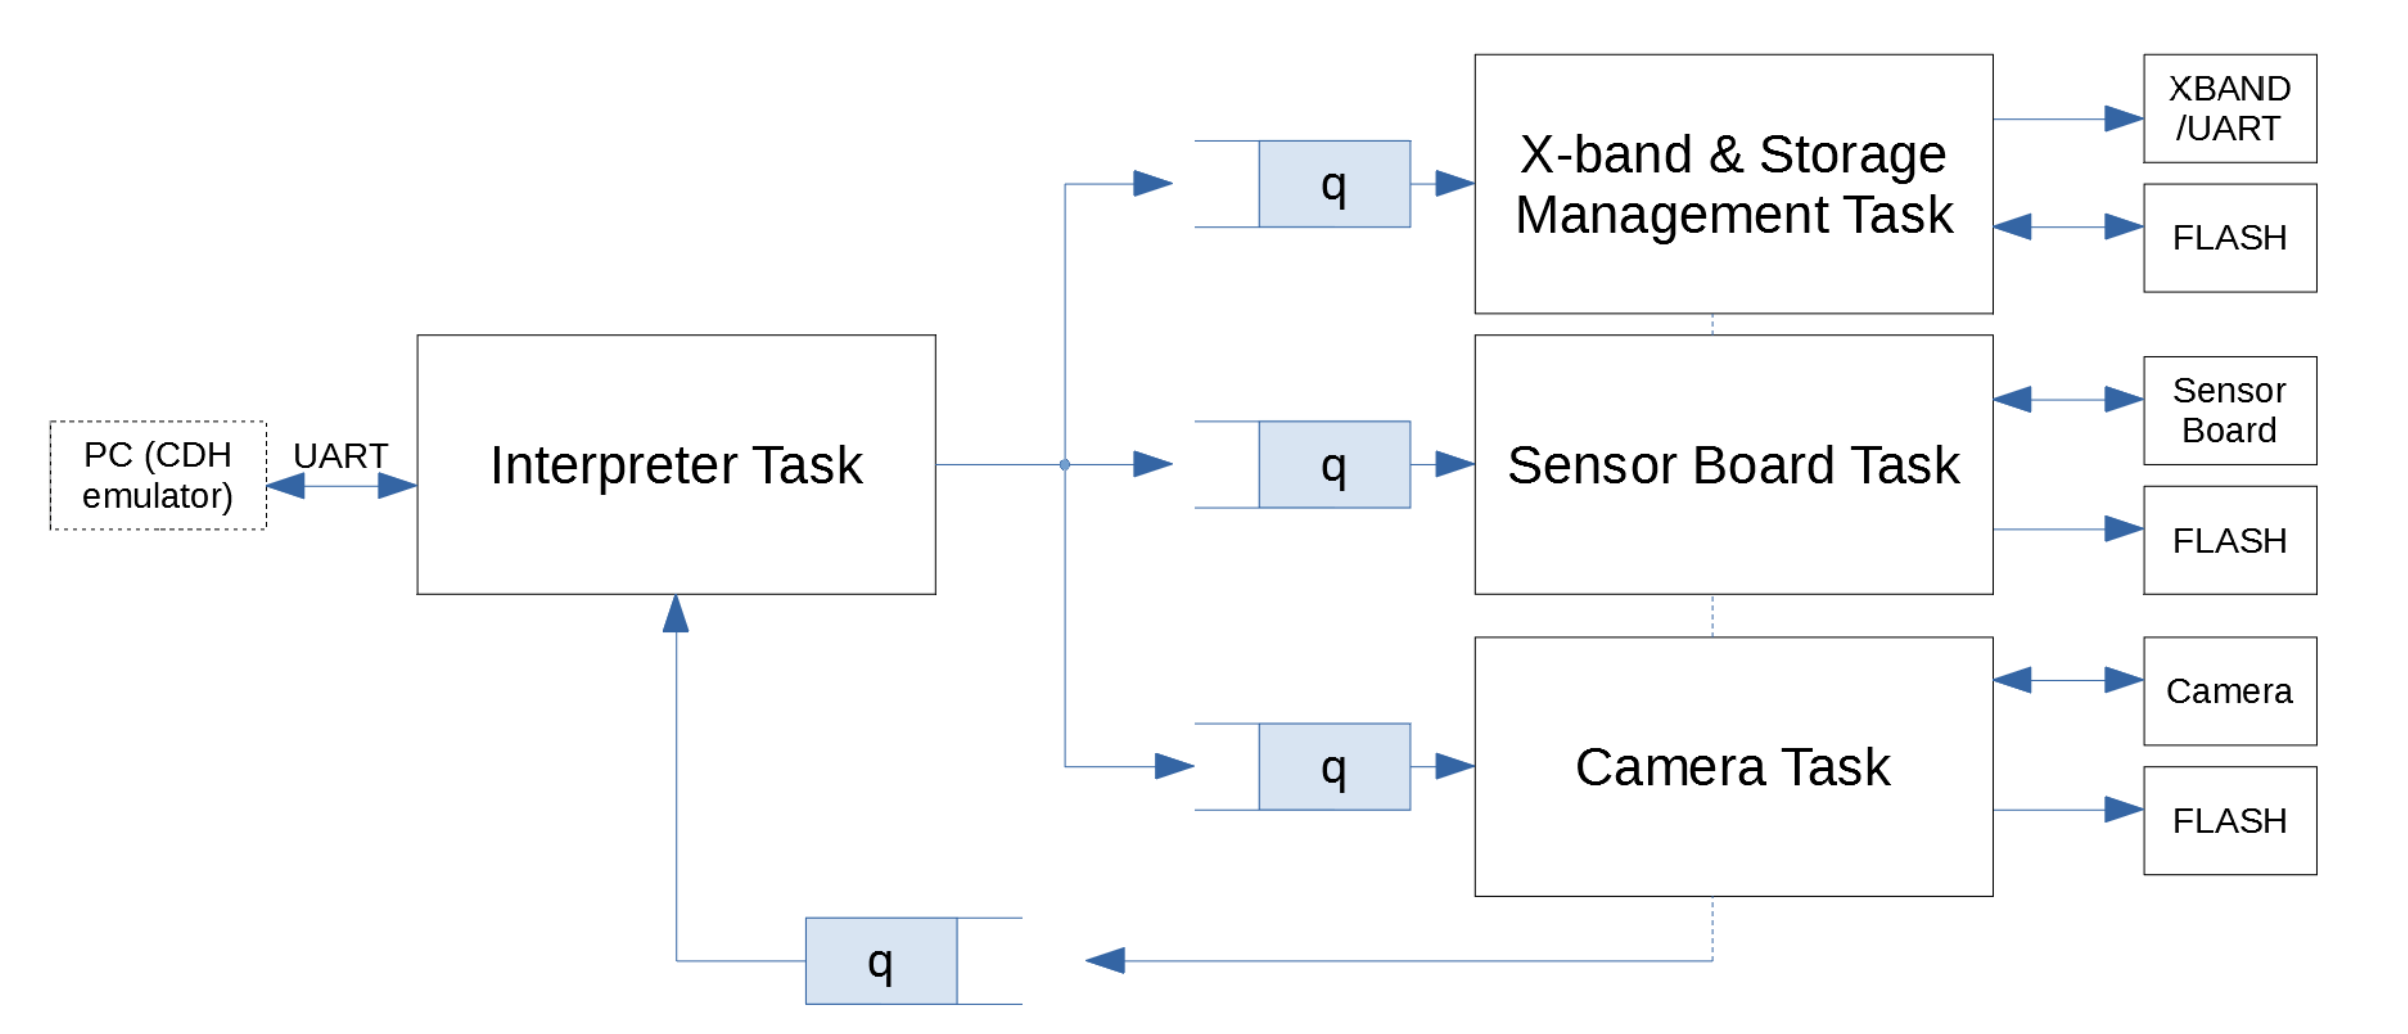
\includegraphics[width=\textwidth]{slike/rtos_zadaci.png}
    \caption{Zadaci programske potpore PDH računala \cite{diplomski_goran_petrak}}
    \label{fig:rtos_zadaci}
\end{figure}

Zadaci međusobno komuniciraju putem redova poruka \engl{message queue}. Zadatak \textit{Interpreter} postavlja parametre za svaki od \textit{device} zadataka (npr. ime datoteke u koju se podaci spremaju, duljinu ekspozicije kamere, itd.) te postavlja poruku s parametrima u red poruka odgovarajućeg zadatka. Kada su postavljeni parametri za sve zadatke, zadatak \textit{Interpreter} spušta svoj prioritet na najniži u sustavu. To omogućuje aktivaciju ostalih zadataka, koji čitaju poruke iz pripadajućih redova i obavljaju svoje poslove. Nakon što neki od zadataka završi s poslom, šalje poruku o uspješnosti u red poruka zadatka \textit{Interpreter}, a zatim biva blokiran čekajući na poruku iz (sada praznog) reda poruka. Kada svi zadaci obave svoj posao, ponovno se aktivira zadatak \textit{Interpreter} i ciklus se ponavlja. Komunikacija između zadataka prikazana je slikom \ref{fig:rtos_zadaci}. Eventualni dijeljeni resursi ne štite se nikakvim posebnim mehanizmima jer je sustav zamišljen tako da se zadaci međusobno ne prekidaju.

Također, u sklopu rada \cite{diplomski_goran_petrak} razvijen je i datotečni sustav za trajnu \textit{Flash} memoriju koja se nalazi na tiskanoj pločici PDH računala. Za rad s datotečnim sustavom razvijene su korisničke funkcije po uzoru na standard POSIX (\textit{Portable Operating System Interface}). Funkcije omogućuju jednostavno pisanje i čitanje datoteka s \textit{Flash} memorije, te se koriste u svim \textit{device} zadacima.